\chapter{Traits}
\label{chap:traits}

This chapter describes the methods of the required operations recognition by the library.\\
\\
Our problem is that the class used as a template has unknown parameters and
methods. Obviously, the library can not classify the purpose of the members of
the class used as template by itself. The solution is to create a new class called \emph{traits}.\\
\\
Traits aggregate all useful types and methods in the way defined by the library.
It is used as a parameter in the templated algorithm and when a method from the traits is called it
returns the result of the method from the mesh implementation or anything that has
a user put into the traits.\\

\textbf{Example:}\\
Implement an algorithm that generates a cube with the centroid in the origin of
the standard coordinate system with edges aligned to $x$,$y$ and $z$ axes and the
length of the edge is $2$. Thus the coordinates of the points are:
\vspace{5mm}
\begin{multicols}{2}
\begin{figure}[H]
\centering
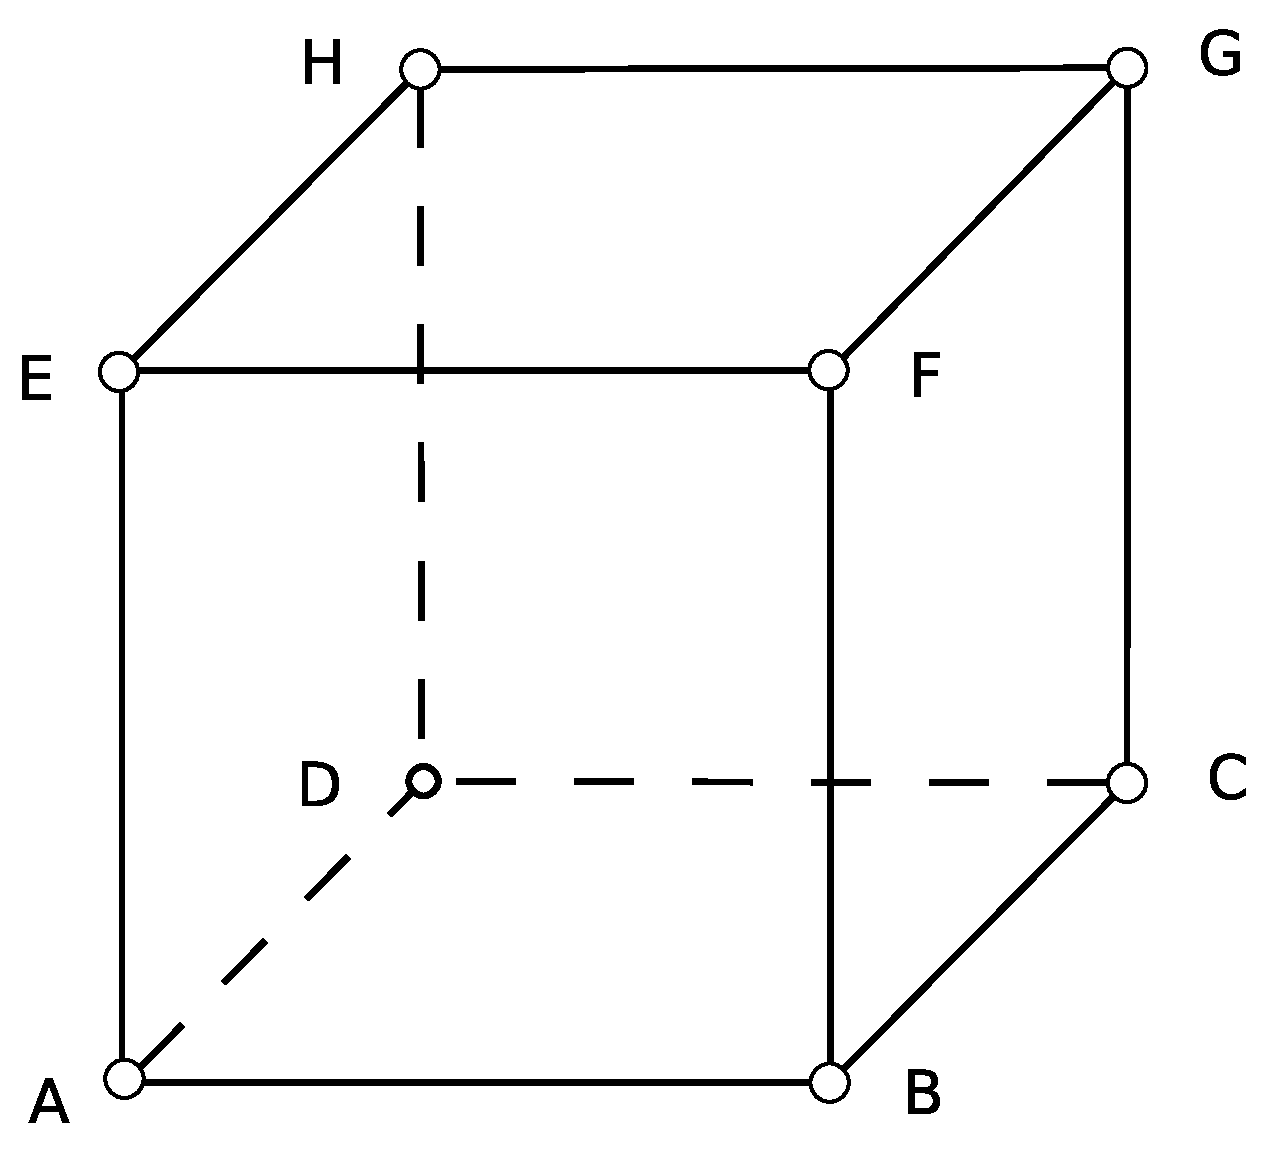
\includegraphics[width=0.6\linewidth]{../img/cube_example.eps}
\end{figure}
\columnbreak
\setlength{\parindent}{0cm}
$A = [-1,-1,-1]$\\
$B = [1,-1,-1]$\\
$C = [1,-1,1]$\\
$D = [-1,-1,1]$\\
$E = [-1,1,-1]$\\
$F = [1,1,-1]$\\
$G = [1,1,1]$\\
$H = [-1,1,1]$\\

\setlength{\parindent}{0.5cm}
\label{mcols:traits_example}

\end{multicols}

The mesh can be assumed as polygonal.\\

\textbf{Solution:}\\
The code will appear as follows:

\lstset { %
belowcaptionskip=1\baselineskip,
breaklines=true,
language=C++,
showstringspaces=false,
basicstyle=\footnotesize\ttfamily,
keywordstyle=\bfseries\color{green!40!black},
commentstyle=\itshape\color{purple!40!black},
identifierstyle=\color{blue},
stringstyle=\color{orange},
backgroundcolor=\color{black!5}
}

\begin{lstlisting}
/**
* \param		m the reference to the mesh
* \returns whether the operation ended successfully
*
* the mesh is assumed as empty. If the mesh is not empty
* it just adds a cube
*/
template <typename TMesh, typename TMesh_traits>
bool generate_cube(TMesh& m)
{
	typedef typename TMesh_traits::Point Point; //coordinates
	typedef typename TMesh_traits::Vertex Vertex; //vertex
	typedef typename TMesh_traits::Face Face; //face type
	
	auto a = Vertex(Point(-1,-1,-1));
	auto b = Vertex(Point(1,-1,-1));
	auto c = Vertex(Point(1,-1,1));
	auto d = Vertex(Point(-1,-1,1));
	auto e = Vertex(Point(-1,1,-1));
	auto f = Vertex(Point(1,1,-1));
	auto g = Vertex(Point(1,1,1));
	auto h = Vertex(Point(-1,1,1));
	
	TMesh_traits::add_vertex(m, a);
	TMesh_traits::add_vertex(m, b);
	TMesh_traits::add_vertex(m, c);
	TMesh_traits::add_vertex(m, d);
	TMesh_traits::add_vertex(m, e);
	TMesh_traits::add_vertex(m, f);
	TMesh_traits::add_vertex(m, g);
	TMesh_traits::add_vertex(m, h);

	TMesh_traits::create_face(m, a, b, c, d);
	TMesh_traits::create_face(m, b, c, g, f);
	TMesh_traits::create_face(m, c, g, h, d);
	TMesh_traits::create_face(m, a, d, h, e);		
	TMesh_traits::create_face(m, e, f, b, a);		
	TMesh_traits::create_face(m, h, g, f, e);
	
	return true; // the cube has been generated succesfully
}
\end{lstlisting}
\label{code:traits}
Without creating an instance, in the class \texttt{TMesh\_Traits} are obtained all
methods and types required for the algorithm. In fact, a type can be named
differently but in the traits class, it must be named following the rules specified
by the interface.\\
\\
Assuming we have class named \texttt{my\_mesh}, the traits class will appear:
\begin{lstlisting}
class my_mesh_traits
{
public:	//the typenames must be visible for the algorithm
	/* TYPES */
	typedef typename Coord_type Point;
	typedef typename My_Vertex Vertex;
	typedef typename My_Face Face;
	typedef typename mesh TMesh;

	/* METHODS */
	inline static Face
	create_face(
		TMesh& m,
		Vertex a,
		Vertex b,
		Vertex c,
		Vertex d)	{/*the implementation*/}
	
	inline static void
	add_vertex(
		TMesh& m,
		Vertex a)	 {/*the implementation*/}
};
\end{lstlisting}